% Regenerates generated/diagram_crossmap-transform-simple-links.{pdf,png} -- the
% crossmap transform figure used as @fig-crossmap-transform in the JCGS paper (issue #3).
%
% Data is demo$simple_links + demo$simple_stats from xmap (xmap#61, 33cd55d):
% 7 source keys -> 6 target keys over 10 weighted links, 2800 either side.
%
% Usage, from src/ (aux files go to a temp dir):
%   f=diagram_crossmap-transform-simple-links
%   tmp=$(mktemp -d) && pdflatex -output-directory=$tmp $f.tex \
%     && cp $tmp/$f.pdf ../generated/ \
%     && pdftoppm -r 400 -png -singlefile ../generated/$f.pdf ../generated/$f

\documentclass[tikz,border=6pt]{standalone}
\usepackage[T1]{fontenc}
\usepackage{lmodern}
\usepackage[scaled=0.92]{helvet}
\usepackage{amsmath,amssymb}
\renewcommand{\familydefault}{\sfdefault}
\usetikzlibrary{arrows.meta}

\definecolor{src}{HTML}{A9C1DE}
\definecolor{tgt}{HTML}{A3BDAE}
\definecolor{zero}{HTML}{BBBBBB}
\definecolor{note}{HTML}{777777}

\tikzset{
  key/.style={rounded corners=2pt, inner sep=1.5pt, minimum height=0.42cm,
    font=\ttfamily\small},
  srckey/.style={key, fill=src, minimum width=1.05cm},
  tgtkey/.style={key, fill=tgt, minimum width=0.7cm},
  frame/.style={line width=1.1pt},
  title/.style={font=\bfseries\large, align=center},
  panel/.style={font=\large},
  link/.style={-{Stealth[length=5pt]}, line width=0.7pt},
  weight/.style={font=\footnotesize, fill=white, inner sep=0.8pt},
  flow/.style={-{Stealth[length=9pt]}, line width=1.6pt},
}

% row geometry shared by every panel: headers span 0..-0.7, rows below
\def\hh{0.7}
\def\rh{0.55}
\newcommand{\rowy}[1]{-\hh-(#1-0.5)*\rh}

\begin{document}
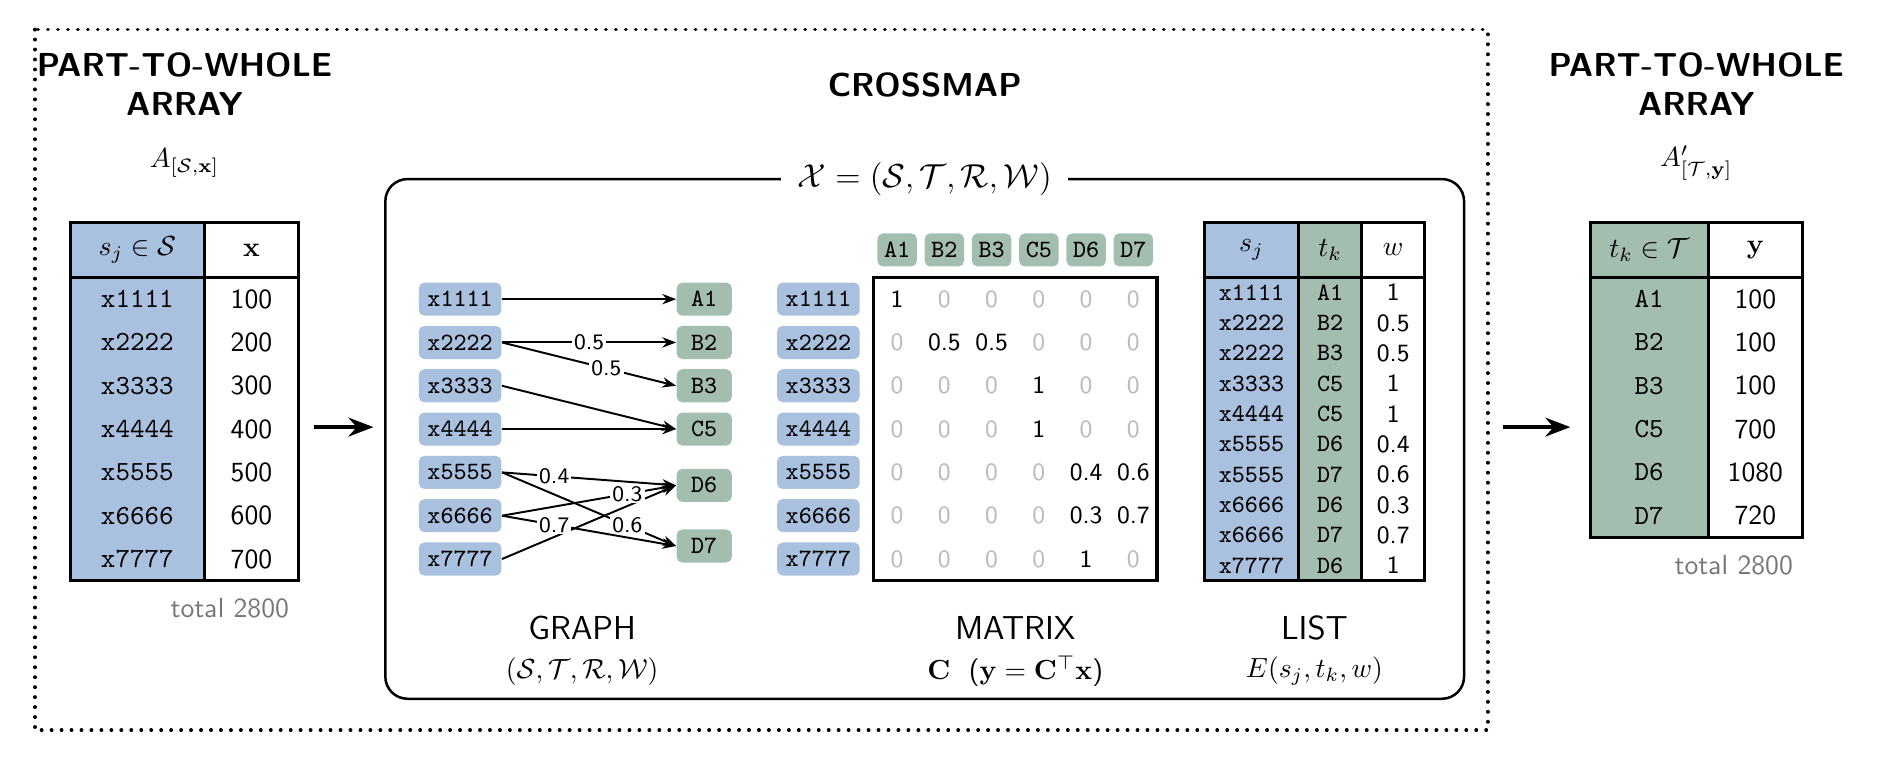
\begin{tikzpicture}

%% ---- reported part-to-whole array --------------------------------------
\node[title] at (1.45,1.75) {PART-TO-WHOLE\\ARRAY};
\node at (1.45,0.75) {$A_{[\mathcal{S},\mathbf{x}]}$};
\fill[src] (0,0) rectangle (1.7,{-\hh-7*\rh});
\node at (0.85,-0.35) {$s_j \in \mathcal{S}$};
\node at (2.3,-0.35) {$\mathbf{x}$};
\foreach \s/\x [count=\i] in
    {x1111/100, x2222/200, x3333/300, x4444/400, x5555/500, x6666/600, x7777/700} {
  \node[font=\ttfamily] at (0.85,{\rowy{\i}}) {\s};
  \node at (2.3,{\rowy{\i}}) {\x};
}
\draw[frame] (0,0) rectangle (2.9,{-\hh-7*\rh});
\draw[frame] (0,-\hh) -- (2.9,-\hh);
\draw[frame] (1.7,0) -- (1.7,{-\hh-7*\rh});
\node[note, anchor=east] at (2.9,{-\hh-7*\rh-0.35}) {total 2800};

\draw[flow] (3.1,-2.6) -- (3.85,-2.6);

%% ---- crossmap ----------------------------------------------------------
\node[title] at (10.85,1.75) {CROSSMAP};
\draw[line width=0.9pt, rounded corners=8pt] (4.0,0.55) rectangle (17.7,-6.05);
\node[fill=white, inner xsep=6pt, font=\large] at (10.85,0.55)
  {$\mathcal{X} = (\mathcal{S},\mathcal{T},\mathcal{R},\mathcal{W})$};

% graph: targets sit near the sources that feed them
\foreach \s [count=\i] in {x1111,x2222,x3333,x4444,x5555,x6666,x7777}
  \node[srckey] (\s) at (4.95,{\rowy{\i}}) {\s};
\foreach \t/\r in {A1/1, B2/2, B3/3, C5/4, D6/5.3, D7/6.7}
  \node[tgtkey] (\t) at (8.05,{\rowy{\r}}) {\t};
\foreach \s/\t in {x1111/A1, x3333/C5, x4444/C5, x7777/D6}
  \draw[link] (\s.east) -- (\t.west);
% fractional links carry their weight; label positions dodge the D6/D7 crossing
\foreach \s/\t/\w/\p in
    {x2222/B2/0.5/0.5, x2222/B3/0.5/0.6,
     x5555/D6/0.4/0.3, x5555/D7/0.6/0.72,
     x6666/D6/0.3/0.72, x6666/D7/0.7/0.3}
  \draw[link] (\s.east) -- node[weight, pos=\p] {\w} (\t.west);

% matrix C: rows are source keys, columns target keys
\foreach \s [count=\i] in {x1111,x2222,x3333,x4444,x5555,x6666,x7777}
  \node[srckey] at (9.5,{\rowy{\i}}) {\s};
\foreach \t [count=\k] in {A1,B2,B3,C5,D6,D7}
  \node[tgtkey, minimum width=0.5cm] at ({10.2+(\k-0.5)*0.6},-0.35) {\t};
\foreach \row [count=\i] in
    {{1,0,0,0,0,0}, {0,0.5,0.5,0,0,0}, {0,0,0,1,0,0}, {0,0,0,1,0,0},
     {0,0,0,0,0.4,0.6}, {0,0,0,0,0.3,0.7}, {0,0,0,0,1,0}} {
  \foreach \c [count=\k] in \row {
    \ifdim\c pt=0pt
      \node[zero, font=\small] at ({10.2+(\k-0.5)*0.6},{\rowy{\i}}) {0};
    \else
      \node[font=\small] at ({10.2+(\k-0.5)*0.6},{\rowy{\i}}) {\c};
    \fi
  }
}
\draw[frame] (10.2,-\hh) rectangle (13.8,{-\hh-7*\rh});

% edge list E: one row per link, same rows as the non-zero cells of C
\def\lh{0.385}
\fill[src] (14.4,0) rectangle (15.6,{-\hh-10*\lh});
\fill[tgt] (15.6,0) rectangle (16.4,{-\hh-10*\lh});
\node at (15.0,-0.35) {$s_j$};
\node at (16.0,-0.35) {$t_k$};
\node at (16.8,-0.35) {$w$};
\foreach \s/\t/\w [count=\i] in
    {x1111/A1/1, x2222/B2/0.5, x2222/B3/0.5, x3333/C5/1, x4444/C5/1,
     x5555/D6/0.4, x5555/D7/0.6, x6666/D6/0.3, x6666/D7/0.7, x7777/D6/1} {
  \node[font=\ttfamily\small] at (15.0,{-\hh-(\i-0.5)*\lh}) {\s};
  \node[font=\ttfamily\small] at (16.0,{-\hh-(\i-0.5)*\lh}) {\t};
  \node[font=\small] at (16.8,{-\hh-(\i-0.5)*\lh}) {\w};
}
\draw[frame] (14.4,0) rectangle (17.2,{-\hh-10*\lh});
\draw[frame] (14.4,-\hh) -- (17.2,-\hh);
\draw[frame] (15.6,0) -- (15.6,{-\hh-10*\lh});
\draw[frame] (16.4,0) -- (16.4,{-\hh-10*\lh});

% panel captions
\node[panel] at (6.5,-5.15) {GRAPH};
\node[panel] at (12.0,-5.15) {MATRIX};
\node[panel] at (15.8,-5.15) {LIST};
\node at (6.5,-5.7) {$(\mathcal{S},\mathcal{T},\mathcal{R},\mathcal{W})$};
\node at (12.0,-5.7) {$\mathbf{C}$ \ ($\mathbf{y} = \mathbf{C}^{\top}\mathbf{x}$)};
\node at (15.8,-5.7) {$E(s_j,t_k,w)$};

%% ---- inputs of the transform -------------------------------------------
\draw[line width=1.3pt, dash pattern=on 0.1pt off 3.5pt, line cap=round]
  (-0.45,2.45) rectangle (18.0,-6.45);

\draw[flow] (18.2,-2.6) -- (19.05,-2.6);

%% ---- imputed part-to-whole array ---------------------------------------
\node[title] at (20.65,1.75) {PART-TO-WHOLE\\ARRAY};
\node at (20.65,0.75) {$A'_{[\mathcal{T},\mathbf{y}]}$};
\fill[tgt] (19.3,0) rectangle (20.8,{-\hh-6*\rh});
\node at (20.05,-0.35) {$t_k \in \mathcal{T}$};
\node at (21.4,-0.35) {$\mathbf{y}$};
\foreach \t/\y [count=\i] in {A1/100, B2/100, B3/100, C5/700, D6/1080, D7/720} {
  \node[font=\ttfamily] at (20.05,{\rowy{\i}}) {\t};
  \node at (21.4,{\rowy{\i}}) {\y};
}
\draw[frame] (19.3,0) rectangle (22.0,{-\hh-6*\rh});
\draw[frame] (19.3,-\hh) -- (22.0,-\hh);
\draw[frame] (20.8,0) -- (20.8,{-\hh-6*\rh});
\node[note, anchor=east] at (22.0,{-\hh-6*\rh-0.35}) {total 2800};

\end{tikzpicture}
\end{document}
